\documentclass[a4paper,12pt]{article}

\usepackage{polyglossia}
\setdefaultlanguage{russian}
\usepackage{fontspec}
\setmainfont{Times New Roman}
\newfontfamily\cyrillicfont{Times New Roman}
\newfontfamily\cyrillicfonttt{FreeMono}

\usepackage[left=2cm, right=2cm, top=2cm, bottom=2cm]{geometry}
\usepackage{graphicx}
\usepackage{float}
\usepackage{wrapfig}
\usepackage{tikz}
\usepackage{amsmath, amsfonts, amssymb}
\usepackage{hyperref}
\hypersetup{
    pdfborder=0 0 0, 
    pdfstartview=FitH, 
    linkcolor=blue, 
    urlcolor=blue, 
    colorlinks=true}

\usepackage{listings}
\lstdefinestyle{codestyle}{
    backgroundcolor=\color{gray!10},
    commentstyle=\color{green!50!black},
    keywordstyle=\color{blue!80!black},
    stringstyle=\color{red!50!black},
    numberstyle=\tiny\color{gray},
    basicstyle=\ttfamily\footnotesize,
    breaklines=true,
    captionpos=b,
    numbers=left,
    numbersep=5pt,
    showstringspaces=false,
    tabsize=2
}
\lstset{style=codestyle}

\usepackage{mdframed}
\newmdenv[
  leftmargin = 0.5em,
  skipabove = 0.5em,
  skipbelow = 0.5em,
  linewidth = 1pt,
  rightline = false,
  topline = false,
  bottomline = false
]{quotebox}

\begin{document}

\begin{titlepage}
    \centering
    {\large Федеральное государственное автономное образовательное учреждение\par}
    {\large высшего образования\par}
    {\bfseries САНКТ-ПЕТЕРБУРГСКИЙ НАЦИОНАЛЬНЫЙ ИССЛЕДОВАТЕЛЬСКИЙ УНИВЕРСИТЕТ ИТМО\par}
    {\bfseries Факультет систем управления и робототехники\par}
    \vfill
    {\Large \bfseries Лабораторная работа №6\par}
    {\Large \bfseries Задачи №1080, 1160, 1450\par}
    \vfill
    
    \begin{flushright}
        Студент: Сайфуллин Д.Р. \\
        Поток: АиСД R23 1.3 \\
        Преподаватель: Тропченко А.А.
    \end{flushright}
    \vfill
    Санкт-Петербург \\
    2025 г.
\end{titlepage}

\section*{Задача №1080. Раскраска карты}
Рассмотрим географическую карту с $N$ странами, занумерованными от 1 до $N$ ($0 < N < 99$). Для каждой страны известны номера соседних стран, т.\,е. имеющих общую границу с данной. Из каждой страны можно попасть в любую другую, перейдя некоторое количество границ. Напишите программу, которая определит, возможно ли покрасить карту только в два цвета — красный и синий — так, что если две страны имеют общую границу, их цвета различаются. Цвет первой страны — красный. Ваша программа должна вывести одну возможную раскраску для остальных стран или сообщить, что такая раскраска невозможна.\\[1em]
\textbf{Исходные данные:}
\begin{quotebox}
    В первой строке записано число $N$. Из следующих $N$ строк $i$-я строка содержит номера стран, с которыми $i$-я страна имеет границу. Каждое целое число в $i$-й строке больше, чем $i$, кроме последнего, которое равно 0 и обозначает конец списка соседей $i$-й страны. Если строка содержит 0, это значит, что $i$-я страна не соединена ни с одной страной с большим номером.
\end{quotebox}
\textbf{Результат:}
\begin{quotebox}
    Вывод содержит ровно одну строку. Если раскраска возможна, эта строка должна содержать список нулей и единиц без разделителей между ними. $i$-я цифра в этой последовательности обозначает цвет $i$-й страны. 0 соответствует красному цвету, единица — синему. Если раскраска невозможна, выведите целое число $-1$.
\end{quotebox}
\subsection*{Рабочий код}
\begin{lstlisting}[language=python]
from collections import deque

def main(adj):
    color = [-1] * (len(adj))
    color[1] = 0
    q = deque([1])

    while q:
        u = q.popleft()
        for v in adj[u]:
            if color[v] == -1:
                color[v] = 1 - color[u]
                q.append(v)
            elif color[v] == color[u]:
                print(-1)
                return
    print(''.join(str(color[i]) for i in range(1, len(adj))))


if __name__ == "__main__":
    n = int(input())
    nodes = [[] for _ in range(n + 1)]
    for i in range(1, n + 1):
        towns = [int(t) for t in input().split()]
        while True:
            x = towns.pop(0)
            if x == 0:
                break
            nodes[i].append(x)
            nodes[x].append(i)
    main(nodes)
\end{lstlisting}
\subsection*{Объяснение алгоритма}
Сначала по входным данным формируется неориентированный граф, в котором вершины соответствуют странам, а ребро соединяет две страны, если у них есть общая граница. Затем нужно проверить, является ли этот граф двудольным при фиксировании первой вершины в «красный» цвет. Для этого запускаем обход в ширину (BFS) из вершины 1, храня массив \texttt{color[1..N]}, инициализированный значением $-1$. В начале $\texttt{color}[1]=0$. При посещении вершины $u$ всех её непокрашенных соседей $v$ красим в цвет $1-\texttt{color}[u]$ и ставим в очередь. Если же мы наталкиваемся на ребро $(u,v)$, где $\texttt{color}[v]=\texttt{color}[u]$, то раскраску в два цвета получить нельзя, и мы выводим «$-1$». В противном случае по завершении BFS в массиве \texttt{color} будет содержаться корректная двухцветная раскраска, которую остаётся просто вывести в виде последовательности нулей и единиц.

\newpage
\section*{Задача №1450. Российские газопроводы}
Сеть российских газопроводов представляет собой $N$ перекачивающих станций, некоторые из которых соединены газопроводами. Для каждого из $M$ газопроводов известны номера станций $A[i]$ и $B[i]$, которые он соединяет, и его прибыльность $C[i]$ - то количество долларов, которое будет ежесуточно приносить в виде налогов перекачка газа по этому газопроводу. Каждая пара станций соединена не более чем одним газопроводом.\\[0.5em]
Сеть была построена советскими инженерами, которые точно знали, что газ поступает из месторождений Украины в Сибирь, а не наоборот. Поэтому все газопроводы являются однонаправленными, т.\,е. для каждого газопровода перекачка газа возможна только в направлении из станции с номером $A[i]$ на станцию с номером $B[i]$. Более того, для любых двух станций $X$ и $Y$ верно, что если возможна перекачка газа из $X$ на $Y$ (возможно, через промежуточные станции), то обратная перекачка из $Y$ на $X$ невозможна. Известно, что газ поступает на начальную станцию с номером $S$ и отгружается потребителям на конечной станции с номером $F$.\\[0.5em]
Президент потребовал от Правительства указать маршрут (то есть линейную последовательность попарно соединённых газопроводами станций) перекачки газа из начальной станции на конечную, причём прибыль этого маршрута должна быть максимальной. Под прибыльностью маршрута понимается суммарная прибыльность входящих в него газопроводов.\\[0.5em]
К сожалению, Президент не учёл того факта, что многие газопроводы изначальной сети уже давно прекратили существование, в результате чего может оказаться, что перекачка газа из начальной станции на конечную вообще невозможна.\\[1em]
\textbf{Исходные данные:}
\begin{quotebox}
    В первой строке записано целое число $N$ ($2 \le N \le 500$) и целое число $M$ ($0 \le M \le 124750$). В каждой из следующих $M$ строк содержатся три целых числа $A[i]$, $B[i]$ ($1 \le A[i], B[i] \le N$) и $C[i]$ ($1 \le C[i] \le 10000$) для соответствующего газопровода. В последней строке записаны два целых числа $S$ и $F$ ($1 \le S, F \le N$; $S \neq F$).
\end{quotebox}
\textbf{Результат:}
\begin{quotebox}
    Если искомый маршрут существует, выведите одно целое число — его максимальную прибыль. Иначе выведите "No solution". 
\end{quotebox}
\subsection*{Рабочий код}
\begin{lstlisting}[language=python]
from collections import deque

def solve(n, edges, s, f):
    graph = [[] for _ in range(n+1)]
    indeg = [0]*(n+1)
    for u, v, c in edges:
        graph[u].append((v, c))
        indeg[v] += 1

    q = deque(i for i in range(1, n+1) if indeg[i] == 0)
    topo = []
    while q:
        u = q.popleft()
        topo.append(u)
        for v, _ in graph[u]:
            indeg[v] -= 1
            if indeg[v] == 0:
                q.append(v)

    NEG = -10**18
    profit = [NEG]*(n+1)
    profit[s] = 0

    for u in topo:
        pu = profit[u]
        if pu == NEG:
            continue
        for v, cost in graph[u]:
            if pu + cost > profit[v]:
                profit[v] = pu + cost

    if profit[f] == NEG:
        print("No solution")
    else:
        print(profit[f])


if __name__ == "__main__":
    n, m = map(int, input().split())
    edges = [tuple(map(int, input().split())) for _ in range(m)]
    s, f = map(int, input().split())
    solve(n, edges, s, f)
\end{lstlisting}
\subsection*{Объяснение алгоритма}
Так как по условию граф ориентированный и ацикличный, достаточно выполнить следующие шаги:
\begin{enumerate}
  \item Построить топологическую сортировку вершин (алгоритм Кана).
  \item Завести массив максимальных прибылей 
  \(\displaystyle \mathrm{dp}[v]=\begin{cases}0,&v=S,\\-\infty,&v\ne S,\end{cases}\)
  где \(S\) — начальная станция.
  \item В порядке топологической сортировки для каждого ребра \((u\to v)\) с прибылью \(c\) выполнять
  \[
    \mathrm{dp}[v]\;=\;\max\{\mathrm{dp}[v],\,\mathrm{dp}[u]+c\}.
  \]
  \item Ответом будет \(\mathrm{dp}[F]\) (или «No solution», если он равен \(-\infty\)).
\end{enumerate}

\newpage
\section*{Задача №1160. Networking}
Andrew is working as system administrator and is planning to establish a new network in his company. There will be $N$ hubs in the company, they can be connected to each other using cables. Since each worker of the company must have access to the whole network, each hub must be accessible by cables from any other hub (possibly via intermediate hubs).\\[0.5em]
Since cables of different types are available and shorter ones are cheaper, it is necessary to make such a plan of hub connections that the maximum length of any single cable is minimized. There is another complication: not every pair of hubs can be directly connected, due to compatibility issues and building geometry limitations. Andrew will provide all necessary information about which hub pairs can be connected and the length of each possible cable.\\[1em]
\textbf{Исходные данные:}
\begin{quotebox}
    The first line contains two integers $N$ and $M$ $(2 \le N \le 10^5,\;0 \le M \le 2\cdot10^5)$ — the number of hubs and the number of possible cables, respectively. Each of the following $M$ lines contains three integers  $u_i,\;v_i,\;w_i$ $(1 \le u_i, v_i \le N,\; 1 \le w_i \le 10^9)$, meaning that hubs $u_i$ and $v_i$ can be joined by a cable of length $w_i$.
\end{quotebox}
\textbf{Результат:}
\begin{quotebox}
    First, output a single integer $L$ — the minimum possible value of the maximum cable length in a spanning plan that connects all hubs.  
    Then output an integer $P$ — the number of cables in your plan.  
    Finally, output $P$ pairs of integers, each pair $u\;v$ indicating that hubs $u$ and $v$ are connected by a cable in your plan. If it is impossible to connect all hubs, output the single line $\texttt{No solution}$ instead.
\end{quotebox}
\subsection*{Рабочий код}
\begin{lstlisting}[language=python]
from collections import deque


def solve(n, edges):
    def find(x):
        while parent[x] != x:
            parent[x] = parent[parent[x]]
            x = parent[x]
        return x
    
    def union(a, b):
        ra, rb = find(a), find(b)
        if ra == rb: return False
        parent[rb] = ra
        return True
    
    parent = list(range(n + 1))
    parent = list(range(n+1))
    def find(x):
        while parent[x] != x:
            parent[x] = parent[parent[x]]
            x = parent[x]
        return x
    def unite(a, b):
        ra, rb = find(a), find(b)
        if ra == rb: 
            return False
        parent[rb] = ra
        return True

    plan = []
    max_len = 0
    for w, u, v in edges:
        if unite(u, v):
            plan.append((u, v))
            if w > max_len:
                max_len = w
            if len(plan) == n-1:
                break

    out = [str(max_len), str(len(plan))]
    for u, v in plan:
        out.append(f"{u} {v}")
    print("\n".join(out))

if __name__ == "__main__":
    n, m = map(int, input().split())
    nodes = []
    for _ in range(m):
        a, b, c = map(int, input().split())
        nodes.append((c, b, a))
    nodes.sort(key=lambda x: x[0])    
    solve(n, nodes)
\end{lstlisting}
\subsection*{Объяснение алгоритма}
Отсортировать все возможные кабели по возрастанию длины и применить алгоритм Крускала с помощью структуры непересекающихся множеств (DSU):
\begin{enumerate}
  \item Перебирать кабели в порядке увеличения длины.
  \item Для каждого кабеля проверять, соединяет ли он два ещё несвязанных хаба; если да — добавить его в план и объединить множества через DSU.
  \item Остановиться, как только все \(N\) хабов окажутся в одной компоненте связности.
\end{enumerate}
Максимальная длина выбранного кабеля в этом остове будет минимально возможным «бутылочным горлышком» сети.

\section*{Статус проверки}
\begin{figure}[H]
    \centering
    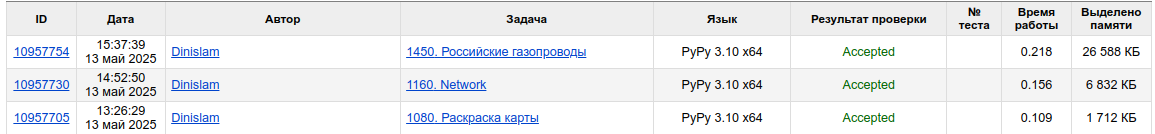
\includegraphics[width=1\textwidth]{check_status.png}
    \caption{Результат проверки}
\end{figure}

\end{document}

